\chapter{性能测试与结果分析}\label{chapter:lab}
本章介绍测试分布式二级哈希表性能的实验,并对实验结果进行了简单的分析。第
\ref{section:assumption}节我阐述了分布式二级哈希表的应用假设,后续章节则说明了
实际的运行环境是怎样决定了系统的设计和实现。很遗憾并没有那样理想的环境,用来对
分布式二级哈希表做一番彻底的测试。因此本章的数据和结论只能在一定程度上反映出分
布式二级哈希表的性能,关于系统的最终评价还要在系统投入实际运行之后,通过检测其
运行情况来得出。

在本次实验中,我测试了分布式二级哈希表对于写入blob的两项性能,包括系统在单位时
间内进行的写入操作数,以及进行一次写入操作的平均时间两项内容。在每个单项测试
中,绘制出了上述性能指标随客户端总写入进程数的变化曲线,其中,客户端总写入进程
数均从1变化到12。这些进程一刻不停的执行写入操作,对于测试平均写入执行时间的实
验,在统计结果时去除了准备数据等无关行为的时间,只计算从开始调用系统接口函数,
到该函数返回的时间;对于测试系统在单位时间内进行写入操作数的实验,则事先将数据
准备好,避免无关操作的影响。对于某一个测试点,比如客户端总写入进程数为N的情
况,这些进程并不是同时开始工作的,而是依次提前10秒开始一刻不停的实行写操作,最
后一个开始的进程总共运行30秒钟,因此倒数第二个开始的进程共运行40秒钟。这样,所
有的进程将同时停止,并且在最后30秒钟同时运行。实验结果即最后30秒钟里,所有进程
的所有写入操作的加权平均值。这样做的目的是希望尽快使系统达到一个稳定状态,记录
该状态下系统的性能。 

分布式二级哈希表读取数据的性能很高。用类似的方法测试分布式二级哈希表读取数据的
能力,读取操作的平均用时在10毫秒以内,并且随客户端并发读取进程数的增加变化不
大。这主要是因为存储服务器上的Redis的读取性能远远高于写入性能。由于读取操作的
失败不会影响数据的完整性,而Redis中所有的数据存储在内存或者应用层虚拟内存中,
因此绝大部分情况下,读取操作需要的数据都可以直接获取,而不必进行硬盘的读操作,
这大大缩短了一次读取操作需要的时间。相反的,写入操作的失败可能影响数据的完整
性,在\ref{section:redis}节中提到过,每次写入操作都会被记录在一个日志文件中,
并且每当对数据进行过一定次数的写入操作后,Redis就会将内存中和用户态虚拟内存中
的数据压缩后存入硬盘。对于像本次实验这种写入数据的速率和规模,触发写入硬盘操作
的频率很高,因此写入操作的性能会远远低于读取操作,这也是本次实验着重探讨写入分
布式二级哈希表写入性能的原因。

本实验的硬件配置参见表\ref{table:config}。其中,配置服务器同时在运行着其他的程
序,因此并没有彻底发挥所有硬件的最大性能。对于客户端的配置,所有数据的索引最大
长度为15字节,数据值的大小为1字节到64KB随机分布,索引和值的内容是随机生成的;
每个客户端进程的线程池共有255个工作线程;$R+W>N$语义按照$(N, W)=(3, 2)$配置。
\begin{table}[htb]
  \centering
  \caption[分布式二级哈希表性能测试实验硬件配置]{分布式二级哈希表性能测试实验
  硬件配置。共设置四台存储服务器,配置同构。其中一台服务器同时作为配置服务器。
  客户端在一台单独的计算机上。所有的存储服务器通过千兆以太网交换机进行连接,客
  户端计算机和存储服务器的连接额外经过一台千兆以太网交换机。}
  \label{table:config}
  \begin{tabular}{p{2cm}|p{5.5cm}|p{5.5cm}}
    \toprule[1.5pt]
    \hei 配置 & \hei 存储服务器 & \hei 客户端 \\
    \midrule[1pt]
    数量 & 4 & 1 \\
    \midrule[1pt]
    内存 & 8GB & 8GB \\
    \midrule[1pt]
    CPU & 4核 Intel(R) Core(TM)2 Q4900 2.66GHz &
    4核 Intel(R) Core(TM) i5 750 2.67GHz \\
    \midrule[1pt]
    硬盘 & 1TB SATA & 1TB SATA \\
    \midrule[1pt]
    操作系统 & Linux 2.6.32-30-server x86\_64 &
    Linux 2.6.38-8-generic x86\_64 \\
    \midrule[1pt]
    网络 & \multicolumn{2}{p{11cm}}{所有的存储服务器通过千兆以太网交换机进行连
    接,客户端计算机和存储服务器的连接额外经过一台千兆以太网交换机。} \\
    \bottomrule[1.5pt]
  \end{tabular}
\end{table}

实验过程中,所有的写入操作均成功返回,没有一次操作失败,即满足第
\ref{section:assumption}节对于操作成功率大于99.999\%的要求,因此在试验结果中将
不再对操作成功率作额外说明。

\section{单位时间写入数据次数}
分布式二级哈希表在稳定运行时,单位时间内完成的写入操作数与客户端并发写入进程数
的关系如图\ref{figure:writethroughput}所示。从图中可以看出,进程数较小时,单位
时间写入数据次数随进程数增加而增加,说明系统的运行能力尚未饱和。当并发写入进程
数达到7个以后,系统单位时间完成的写入数据次数不再随写入进程数增加而增大,而是
稳定在一个固定数值,即每台服务器平均每秒最多处理的写入操作数约为30。
\begin{figure}[htb]
  \centering
  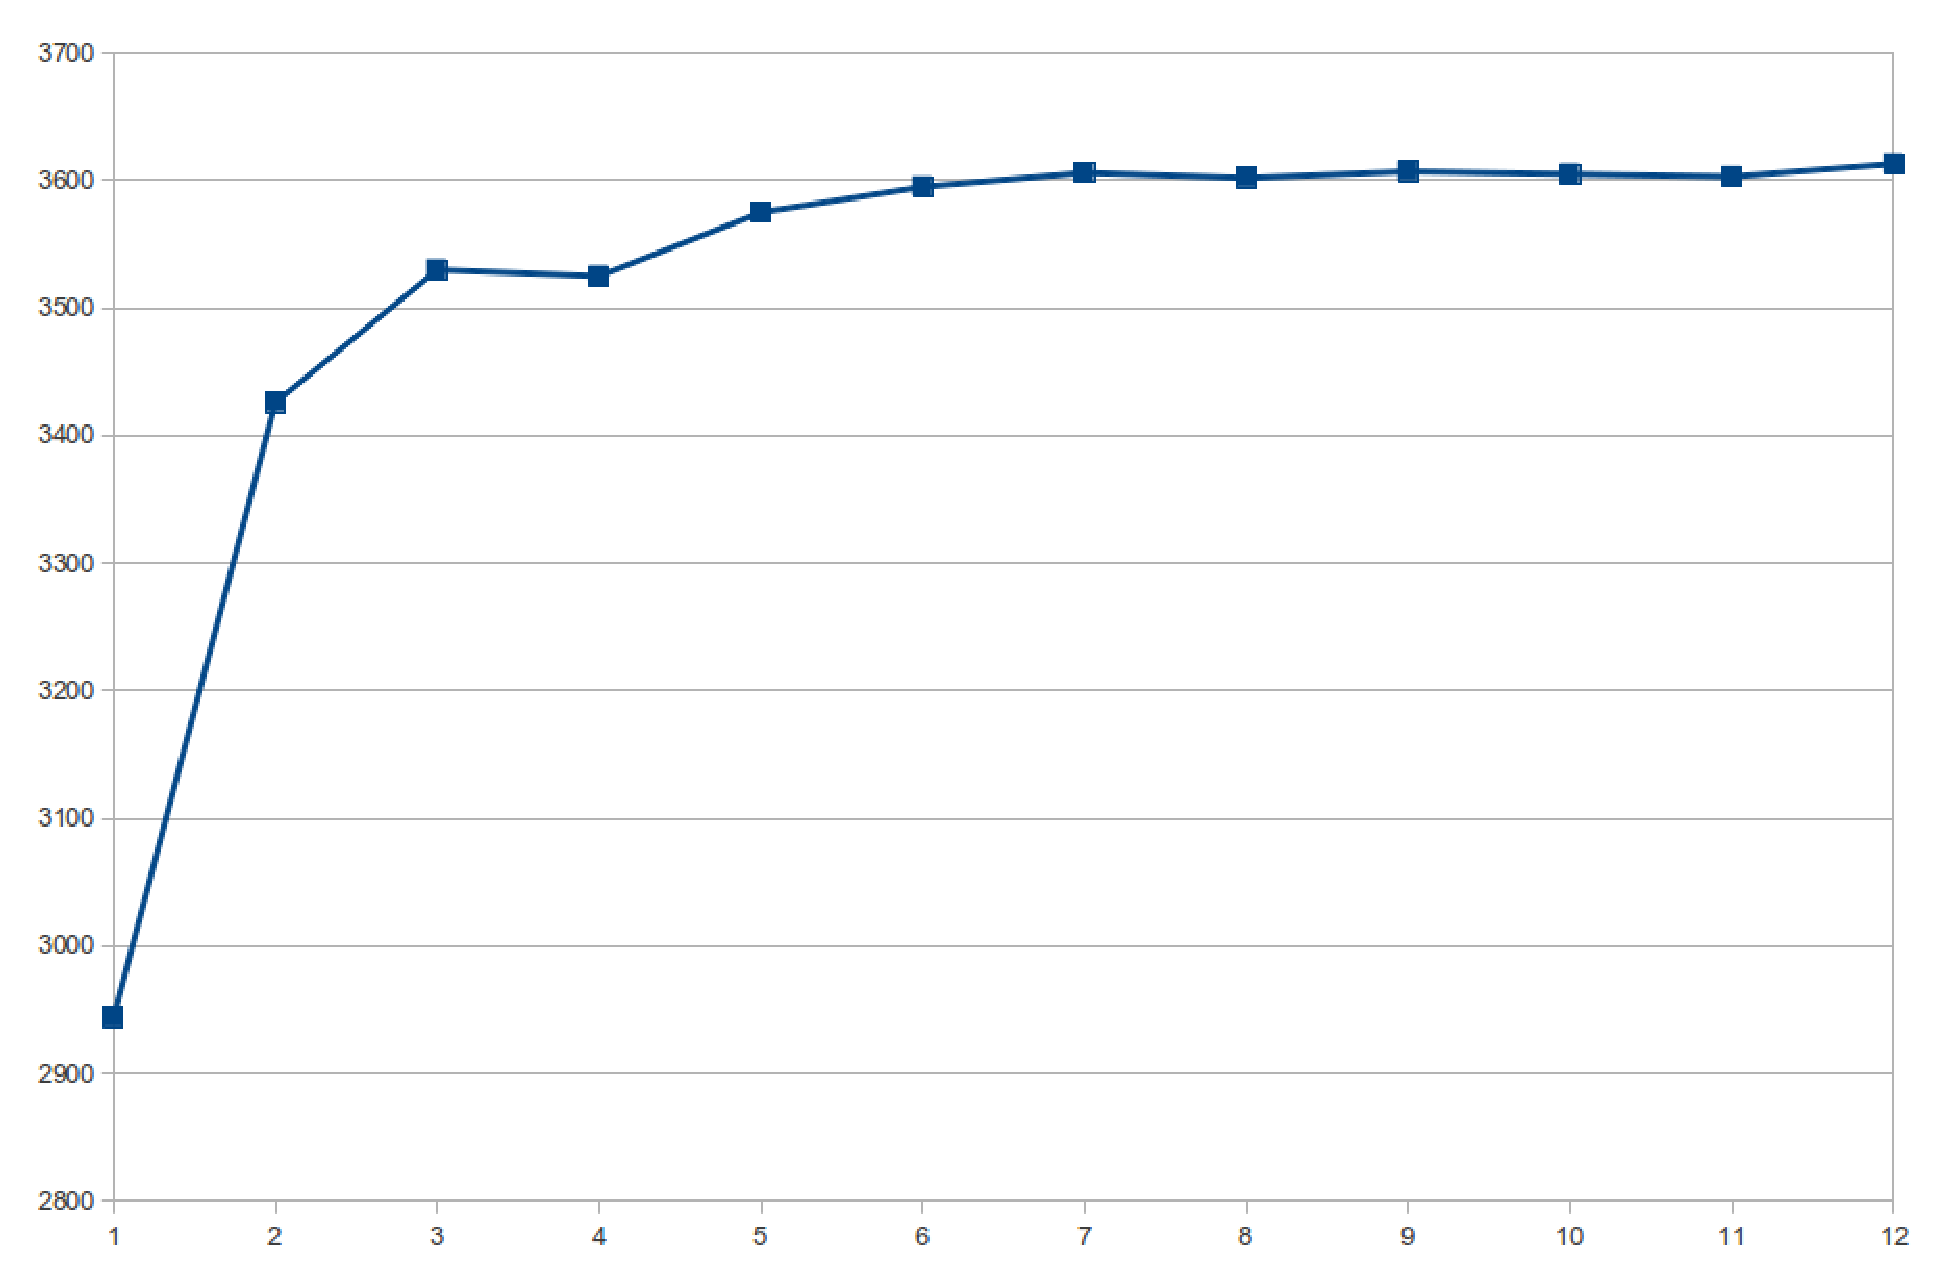
\includegraphics[width=1.0\linewidth]{writethroughput}
  \caption[分布式二级哈希表单位时间写入数据次数]{分布式二级哈希表单位时间写入
  数据次数与并发写入进程数的关系。横轴代表写入进程数,纵轴代表半分钟内系统完成
  的写入请求总数。每台服务器平均每秒最多处理的写入操作数约为30。}
  \label{figure:writethroughput}
\end{figure}

由于实验只计算最后半分钟所有写进程同时工作时的数值,而进程又是逐个加入的,因此
当进程数较少时,系统的最后半分钟并未达到饱和运行状态。当进程数比较多时,在最后
半分钟的运行过程中,系统已经饱和,因此单位时间内的写入操作次数不再发生变化。当
系统进入饱和状态时,主要的制约因素是内存中的数据一直在向硬盘中写入。普通
7200RPM SATA硬盘的IOPS约为90\footnote{http://en.wikipedia.org/wiki/IOPS},而对
于一个数据的写入需要进行三次硬盘读写操作:
\begin{enumerate}
  \item 将内存或用户态虚拟内存中某块缓存数据写入硬盘。
  \item 将硬盘上存储目标数据的本地哈希表读出。
  \item 额外申请内存扩大此哈希表,写入目标数据,这必然引发内存或用户态虚拟内存
  中另一块数据写入硬盘。
\end{enumerate}
因此每台服务器平均每秒最多处理的写入操作数约为30,已经达到了当前系统实现和硬件
配置的极限。

\section{平均写入时间}
分布式二级哈希表在稳定运行时,写入操作的平均执行时间与客户端并发写入进程数的关
系如图\ref{figure:writeresponse}所示。从图中可以看出,写入操作的平均执行时间随
客户端并发写入进程数近似线性增加。
\begin{figure}[htb]
  \centering
  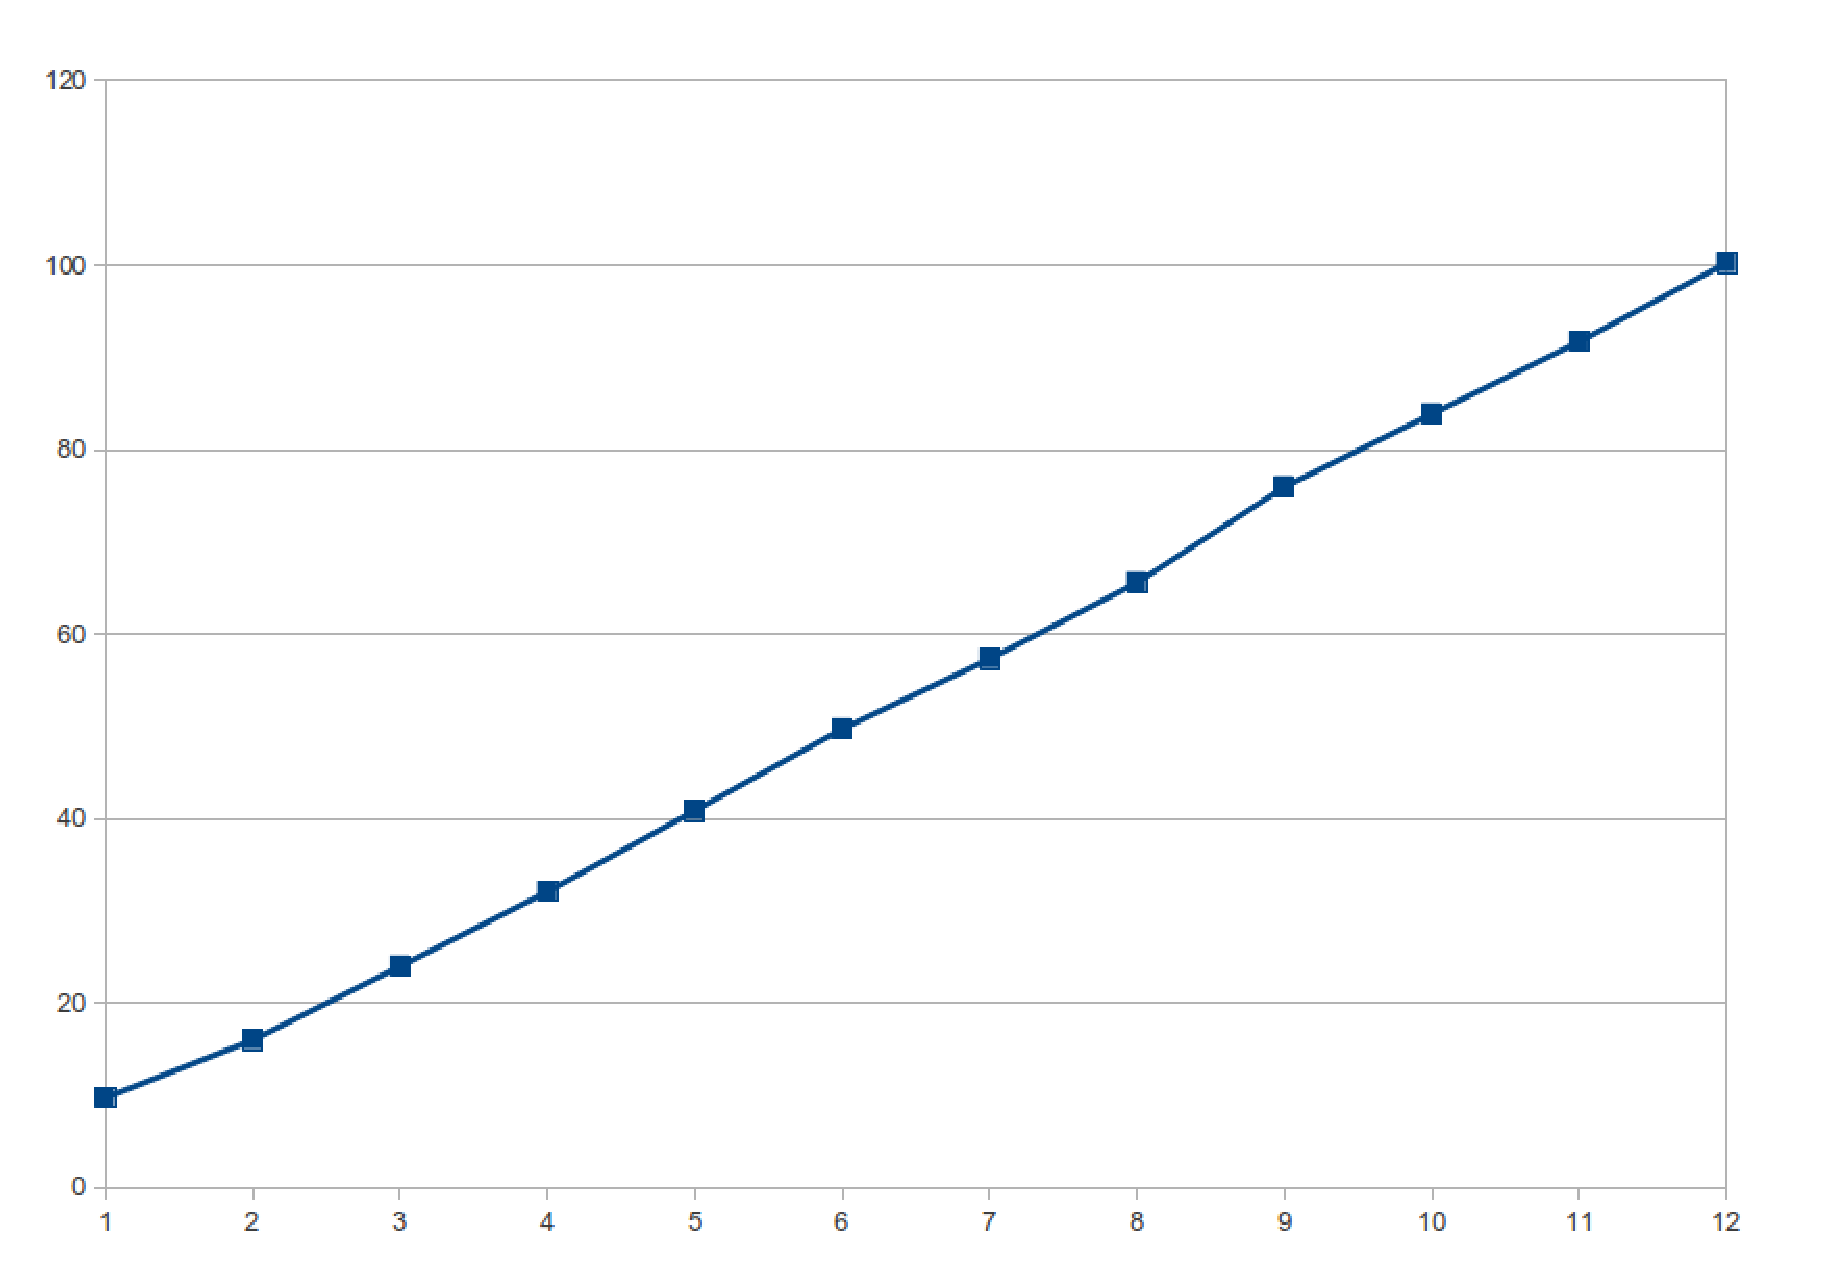
\includegraphics[width=1.0\linewidth]{writeresponse}
  \caption[分布式二级哈希表平均写入时间]{分布式二级哈希表平均写入时间与客户端
  并发写入进程数的关系。横轴代表写入进程数,纵轴代表平均写入时间,单位是毫秒。
  平均写入时间随写入进程数增加近似线性增大。}
  \label{figure:writeresponse}
\end{figure}

这个有趣的结果并非处于偶然,却很难给出一个直观的解释。为了探究其中的原因,我做
了进一步的实验,将每一个操作分解,统计各个子操作的时间,得到图
\ref{figure:linear}所示的结果。其中,蓝线、红线、黄线均表示网络通信的时间,并
且红线与黄线之和跟绿线的差值即为客户端本地计算的开销,比如线程的调度等。绿线与
蓝线的和与深红线的差值也表示本地开销。比较意外的是,几乎所有子操作的时间都随写
进程数线性增加,因此基本可以断定瓶颈在于客户端而不是网络带宽或者存储服务器的处
理能力。图\ref{figure:writethroughput}已经说明当线程数不大于4个时,存储服务器
并没达到饱和状态,因此黄线呈线性变化的原因应该是客户端读取socket结果的时间呈线
性变化,那么一种合理的解释是,由于每个写进程的线程池包含255个线程,客户端线程
调度的开销比较大,以至于客户端的每一个子操作都受到了影响,包括本地计算和网络数
据传输等操作,因为这些操作的进程与线程池中的线程是一起被操作系统所调度的
\footnote{http://en.wikipedia.org/wiki/NPTL}。随着写进程数增加,线程总数正比增
大,单位时间内每一个线程被调度到的次数反比减小,因此每一个操作的执行时间都正比
增大。当然,进一步的分析还需要后续实验做深入的验证和讨论。
\begin{figure}[htb]
  \centering
  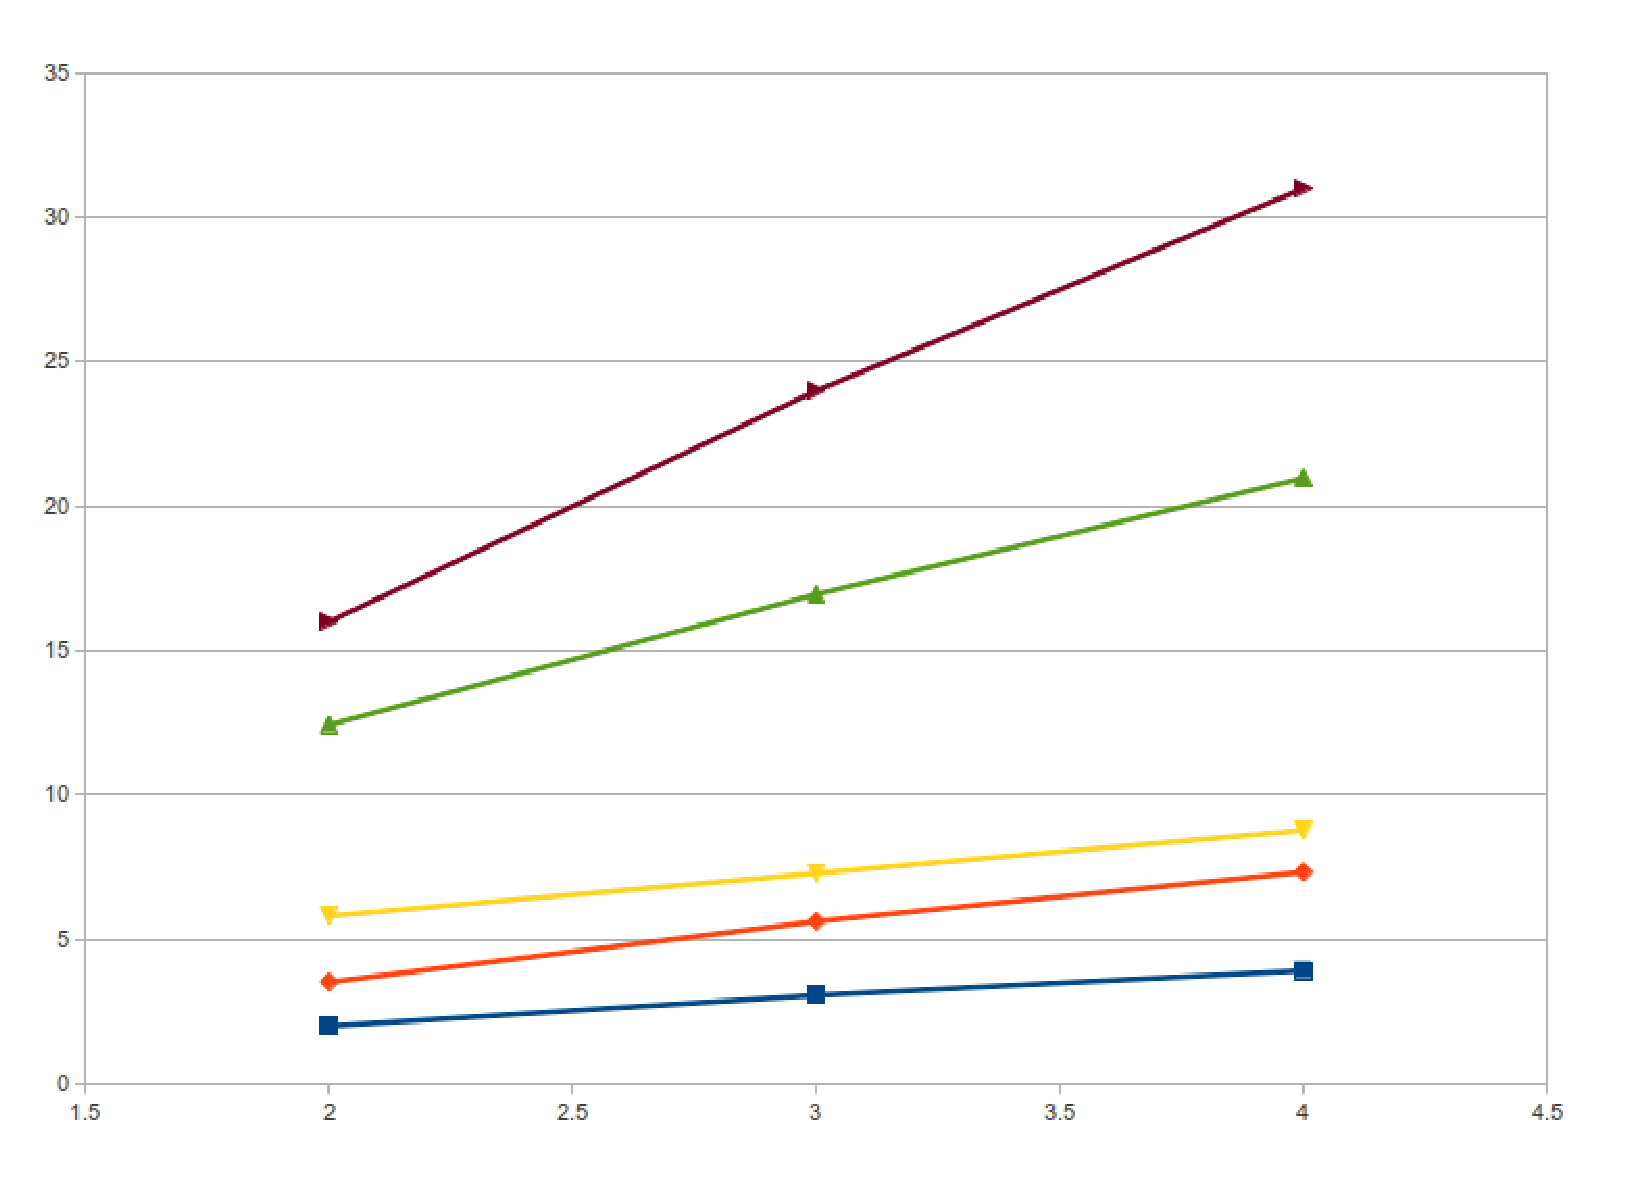
\includegraphics[width=1.0\linewidth]{linear}
  \caption[分布式二级哈希表平均写入时间拆分]{分布式二级哈希表平均写入时间拆
  分。横轴代表写入客户端并发写入进程数,纵轴代表平均写入时间,单位是毫秒。
  蓝线是客户端从配置服务器获取目标存储服务器IP地址平均时间,红线是客户端向存
  储服务器发送指令和数据的平均时间,黄线是客户端从发送完指令和数据到读到存储
  服务器传回结果数据的平均时间,绿线是任务进入线程池到读到结果的平均时间,深
  红线是上层应用调用接口函数到得到返回值的平均时间。各个子操作的时间均随客户
  端写入线程数近似线性增加。}
  \label{figure:linear}
\end{figure}
